
\documentclass{beamer}
\usetheme{Berlin}
\usecolortheme{default}

\usepackage{cmap}                   % поиск в PDF
\usepackage{braket}
\usepackage[T2A]{fontenc}           % кодировка
\usepackage{mathtext}               % русские буквы в формулах
\usepackage[utf8]{inputenc}         % кодировка исходного текста
\usepackage[english,russian]{babel} % локализация и переносы

\title{Реализация квантового компьютера на ионной ловушке}
\subtitle{Вопрос по выбору к ГКЭ, январь 2022}
\author{Станислав Сидельников Б01-908, Егор Батарин Б01-906}
\institute{Московский физико-технический институт}
\date{}

\begin{document}
    
    \begin{frame}
        \titlepage
    \end{frame}

    \begin{frame}{Содержание}

        \begin{itemize}
            \item Введение в квантовые вычисления

                \begin{itemize}
                    \item Классический бит и квантовый бит
                    \item 

                \end{itemize}

            \item Принцип работы ионной ловушки

                \begin{itemize}
                    \item{Захват иона}
                    \item{Доплеровское охлаждение}
                \end{itemize}

            \item Хранение состояний

            \item
        \end{itemize}

    \end{frame}

	\begin{frame}{Введение в квантовые вычисления}
	\framesubtitle{Классический бит и квантовый бит}
	Классический бит: $0$ или $1$ - два состояния.
	\vspace{3mm}
	
	Квантовый бит: $\ket{\psi} = \alpha\ket{0} + \beta\ket{1}$, $\alpha,\beta \in \mathbb{C}$, $|\alpha|^2 + |\beta|^2 = 1$ - бесконечно много состояний?
	\vspace{3mm}
	
	Представление на сфере Блоха: $\ket{\psi} = e^{i\gamma}\left(  \cos{\frac{\theta}{2}}\ket{0}+e^{i\phi}\sin{\frac{\theta}{2}} \ket{1}  \right) \sim \cos{\frac{\theta}{2}}\ket{0}+e^{i\phi}\sin{\frac{\theta}{2}} \ket{1} $,
	
	где $\gamma, \theta$ и $\phi$ - действительные числа.
	\end{frame}
    
    \begin{frame}{Введение в квантовые вычисления}
    \framesubtitle{Классический бит и квантовый бит}
    
    \begin{figure}[]
    	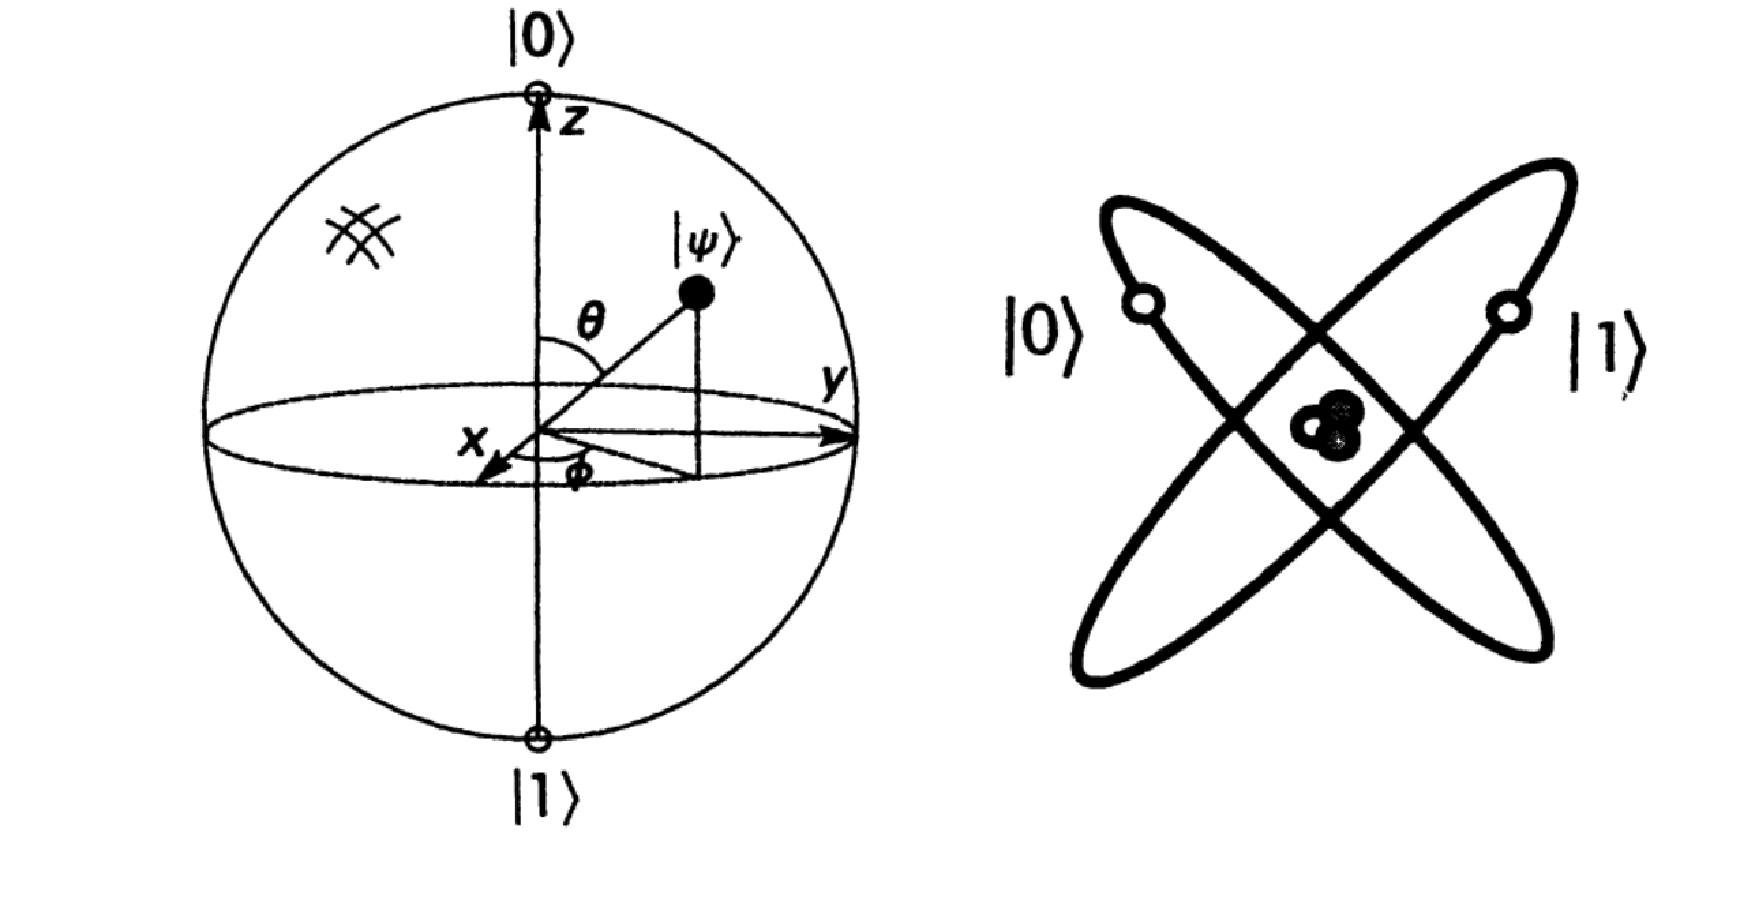
\includegraphics[width=\linewidth]{media/qubits.pdf}
    \end{figure}
    
	\end{frame}

\end{document}